%
% homogen.tex -- homogene Koordinaten
%
% (c) 2018 Prof Dr Andreas Müller, Hochschule Rapperswil
%
\subsection{Homogene Koordinaten\label{section:homogene koordinaten}}
Wir wollen das Abbildungs-Problem für eine einzelne Kamera lösen.
Ein Punkt im dreidimensionalen Raum wird durch seine drei Koordinaten
$(x,y,z)$ beschrieben.
Wir nennen einen solchen Punkt auch {\em Weltpunkt} und seine Koordinaten
die {\em Weltkoordinaten}.
\index{Weltpunkt}%
\index{Weltkoordinaten}%
Er wird abgebildet auf einen {\em Bildpunkt} auf dem Kamera-Chip mit
Pixel-Koordinaten, auch {\em Bildkoordinaten}.
\index{Bildpunkt}%
\index{Bildkoordinaten}%
\begin{aufgabe}[Abbildungsproblem für Kameras]
Gegeben die Koordinaten eines Weltpunktes, berechne die Bildkoordinaten
für eine beliebige Kamera.
\end{aufgabe}
Es ist klar, dass alle Punkte auf einem Strahl durch die Kamera auf den
gleichen Bildpunkt abgebildet werden.
Gesucht ist also eine mathematische Beschreibung, die solche Strahlung
zu beschreiben gestattet.
Dies sind die {\em homogenen Koordinaten}.

\subsubsection{Strahlensatz}
\begin{figure}
\centering
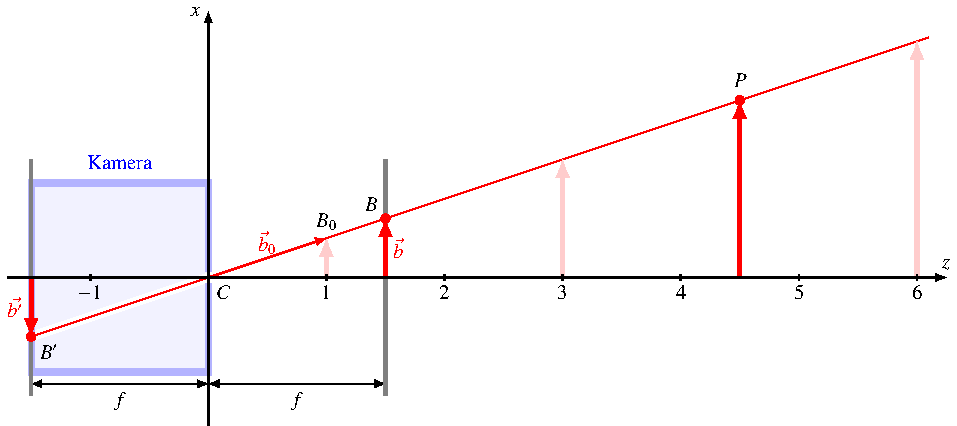
\includegraphics{applications/kamera/strahlensatz.pdf}
\caption{Strahlensatz und Abbildung eines Punktes $P$ durch eine Lochkamera
mit Brennweite $f$.
\label{skript:kamera:strahlensatz}}
\end{figure}
In Abbildung~\ref{skript:kamera:strahlensatz} ist illustriert, wie
der Punkt $P$ durch die blau angedeutete Lochkamera auf den Punkt $B'$
abgebildet wird.
Das Loch befindet sich im Punkt $C$, die Kamera hat die Brennweite $f$.
Der Pfeil von der $z$-Achse zum Punkt $P$ der Länge $x(z)$ wird
auf den kopfstehenden Pfeil von der $z$-Achse zum Punkt $B'$ abgebildet.
Das Abbildungsproblem ist gelöst, wenn wir die Länge des Vektors $\vec{b'}$
bestimmen können.
Da $\vec{b}'=-\vec{b}$ ist das gleichbedeutend damit, den Vektor $\vec{b}$
zu bestimmen.

Alle Punkte auf der roten Geraden durch $C$ und $P$ werden von der Kamera
auf den gleichen Punkt $B'$ abgebildet.
Die Gerade besteht aus den Punkte mit Ortsvektoren, die Vielfache des
Vektors $\vec{b}_0=\overrightarrow{CB_0}$ sind.
Alle Punkte sind also Vielfache des Vektors 
\[
\vec{b}_0
=
\overrightarrow{CB_0}
=
\begin{pmatrix}x(B_0)\\1\end{pmatrix}.
\]
Auch der Ortsvektor des Bildpunktes $B$ in der Fokusebene ist ein Vielfaches 
von $\vec{b}_0$, nämlich
\[
\overrightarrow{CB} =
=
\begin{pmatrix}x(B)\\f\end{pmatrix}
=
f \cdot
\begin{pmatrix}x(B_0)\\1\end{pmatrix}.
\]
Unabhängig von der Brennweite können als alle Bildpunkte durch 
den Vektor $\vec{b}_0$ dargestellt werden.
Dies suggeriert, dass wir als Koordinatensystem für die Punkte in der
Brennebene nicht einfach nur die Länge der Strecke von der $z$-Achse 
zum Punkt $B$ verwenden sollen, sondern zweidimensionale Vektoren.
Die Länge der genannten Strecke finden wird dann, indem wir den Vektor
so skalieren, dass die zweite Komponenten $f$ wird.

\begin{definition}
Wir nennen Zahlenpaare $(x_0,x_1)$ {\em homogene Koordinaten} für die
Punkte einer Geraden, wenn mindestens eine der Komponenten von $0$
verschieden ist.
Die inhomogenen (gewöhnlichen) Koordinate eines Punktes mit
homogenen Koordinaten $(x_0,x_1)$ mit $x_1\ne 0$ ist $x_0/x_1$.
\end{definition}
\index{homogene Koordinaten}%
Man beachte, dass den homogenen Koordinaten $(1,0)$ keine gewöhnlichen
Koordinaten zugeordnet sind.
Sie beschreiben einen Punkte auf der $x$-Achse von
Abbildung~\ref{skript:kamera:strahlensatz}, doch dieser Punkt kann
von der Kamera gar nicht abgebildet werden.
Man nennt diesen Punkt manchmal auch den {\em unendlich fernen Punkt} der
Geraden.
\index{unendlich ferner Punkt}%

In homogenen Koordinaten lässt sich das Abbildungsproblem also ganz
einfach lösen. 
Der Punkt $P$ mit Koordinaten $(x,z)$ wird abgebildet auf den Punkt
mit homogenen Koordinaten $(x,z)$.
Um die inhomogene Koordinate mit in einer Kamera mit Brennweite $f$ zu
berechnen, setzen wir einfach $f\cdot x/z$ ein.

Auf den Mittelpunkt des Bildes werden alle Punkte der $z$-Achse
in Abbildung~\ref{skript:kamera:strahlensatz} abgebildet.
Die homogenen Koordinaten dieses Punktes sind $(0,1)$, dies ist
auch der Richtungsvektor der Blickrichtung der Kamera.

\subsubsection{Zentralprojektion auf eine Ebene}
\begin{figure}
\centering
\caption{Abbildung von Punkten des dreidimensionalen Raumes durch eine
Lochkamera.
\label{skript:kamera:lochkamera}}
\end{figure}
Bisher haben wir eine eindimensionale Kamera studiert, dafür gibt
es durchaus bereits Anwendungen, zum Beispiel Scanner mit linearem
Bildsensor.
Aber natürlich
interessieren uns vor allem realistischere Kameras mit zweidimensionalem
Sensor.
Dazu müssen wir das Konzept der homogenen Koordinaten auf einen
dreidimensionalen Raum ausdehen.

\begin{definition}
Wir nennen Zahlentripel $(x_0,x_1,x_2)$ {\em homogene Koordinaten}
für die Punkte einer Ebene, wenn mindestens eine der Komponenten von $0$
verschieden sind.
Die inhomogenen Koordinaten eines Punktes mit homogenenen Koordinaten
$(x_0,x_1,x_2)$ mit $x_2\ne 0$ sind $(x_0/x_2,x_1/x_2)$.
\end{definition}

Wir stellen uns also wieder vor, eine Lochkamera im Ursprung des
Koordinatensystems platziert zu haben mit Blickrichtung entlang der
$z$-Achse.
Die inhomogenen Koordinaten des Punktes $P=(x,y,z)$ können wir dann
wieder als homogene Koordinaten einer Ebene betrachten.
Die Abbildung durch die Lochkamera mit Brennweite ist dann wieder sehr
einfach zu lösen: der Punkt $P$ wird auf den Punkt mit homogenen Koordinaten
$(x,y,z)$ abgebildet.
Die Koordinaten in der Brennebene einer Kamera mit Brennweite $f$ sind dann
$f\cdot (x/z, y/z)$.

Die Punkte mit $z=0$ können nicht abgebildet werden.
Wenn die $z$-Koordinaten eines Punktes gegen $0$ geht, bewegt sich sein
Bild in der Brennebene der Lochkamera nach aussen gegen unendlich.
Man nennt diese Punkte daher manchmal auch unendlich ferne Punkte.
Da sie ausserdem eine lineare Gleichung erfüllen, kann man die Menge dieser
Punkte auch die {\em unendlich ferne Gerade} nennen.
\index{unendlich ferne Gerade}%


